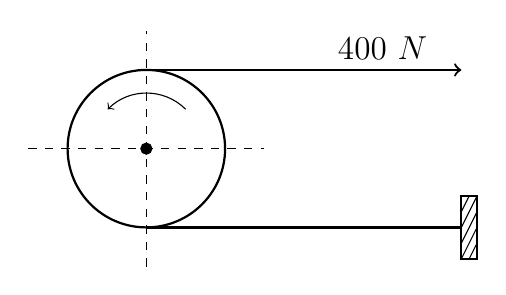
\begin{tikzpicture}
    % Draw the circle
    \draw[thick] (0,0) circle(1);
    
    % Draw the center point and dashed lines
    \draw[dashed] (-1.5,0) -- (1.5,0);
    \draw[dashed] (0,-1.5) -- (0,1.5);
    \filldraw (0,0) circle (2pt);

    % Draw the rotational arrow
    \draw[->] (0.5,0.5) arc[start angle=45, end angle=135, radius=0.7];

    % Draw the 400 N force arrow
    \draw[thick, ->] (0,1) -- (4,1) node[near end, above] {\large $400\ \text{N}$};

    % Draw the fixed support on the right
    \draw[thick] (0, -1) -- (4, -1);
    \begin{scope}
    % Clip to the rectangle
    \clip (4.2, -1.4) rectangle (4, -0.6);
    % Draw diagonal lines
    \foreach \x in {3,3.1,...,5} { % Correct range and ensure semicolon
        \draw[thin] (\x,-2) -- (\x+1,0); % Add semicolon
    }
\end{scope}

% Outline the rectangle
\draw[thick] (4.2, -1.4) rectangle (4, -0.6);
\end{tikzpicture}
